\section{Remote sensing}


\subsection{Electromagnetic radiation}
Satellites all work the same way: they are flying machines that carry a camera. The camera has one or more sensors, each of which can observe some part of the electromagnetic spectrum.
Radar satellites have their own 'light' source: they actively send out radio-radiation and collect the reflection.

\begin{itemize}
    \item Optical
    \item Radar: not hindered by clouds. Good for flood-detection
    \item Microwave: good for atmospheric observation
\end{itemize}


\begin{figure}[H]
    \caption{Frequencies capable of penetrating the atmosphere}
    \centering
      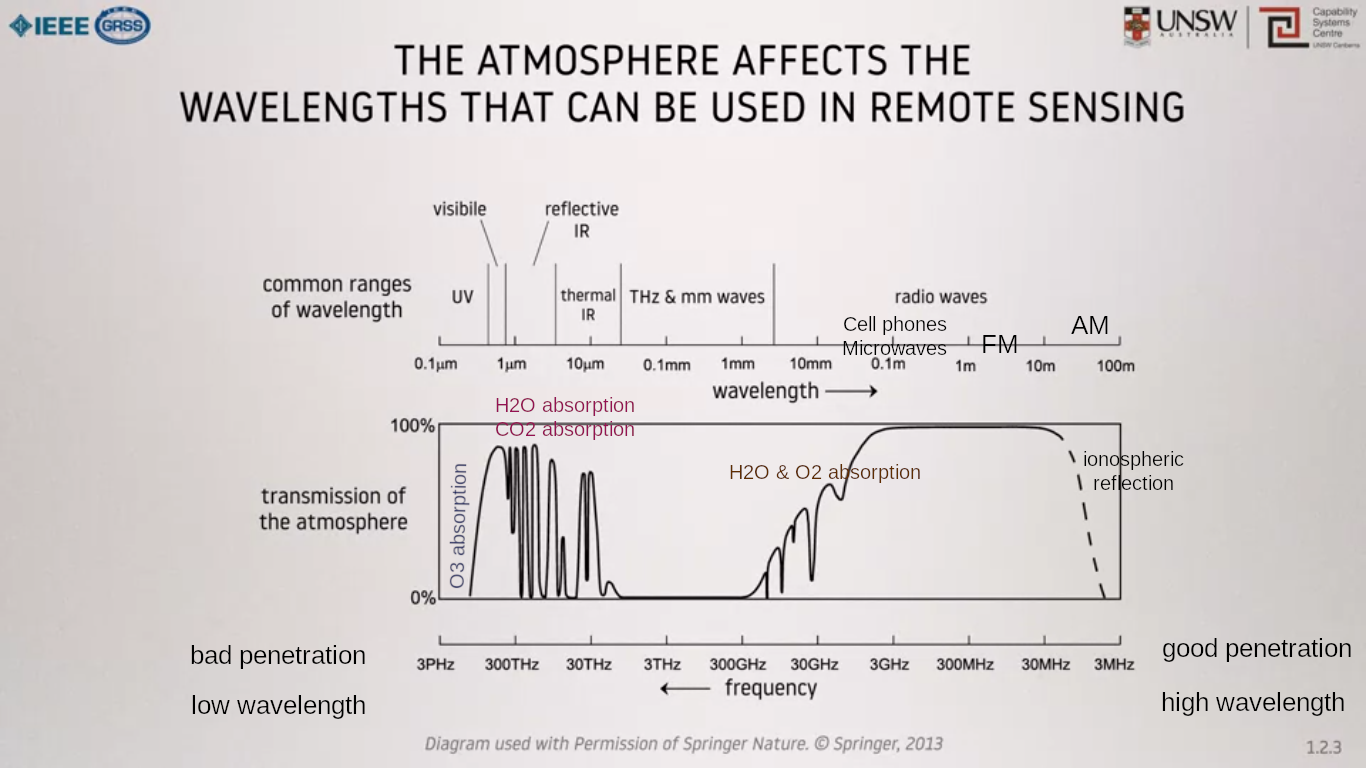
\includegraphics[width=0.75\textwidth]{images/rs_atmospheric_absorption.png}
\end{figure}

\begin{figure}[H]
    \caption{Guide to the selection of frequencies in VIS \& NIR range}
    \centering
      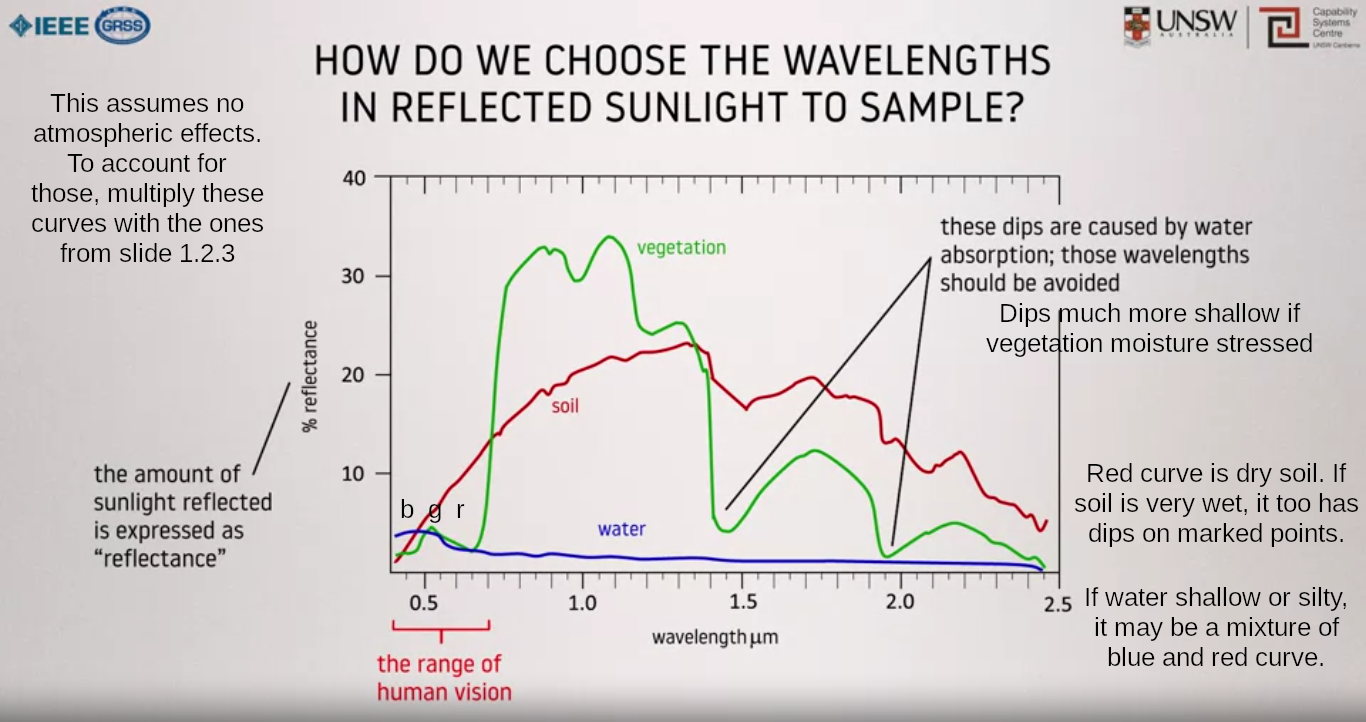
\includegraphics[width=0.75\textwidth]{images/rs_vis_nir_curves.png}
\end{figure}

\begin{figure}[H]
    \caption{Example of important groups in VIS \& NIR}
    \centering
      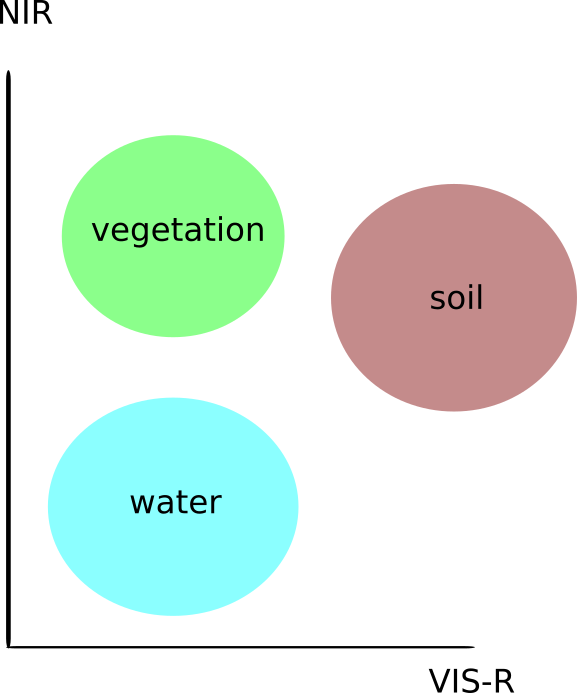
\includegraphics[width=0.35\textwidth]{images/rs_vis_nir_groups.png}
\end{figure}


\subsection{Radar}
Radar is a little different from the optical VIS / NIR satellites.
The earth does not emit any radar-radiation (naturally, only a few pulsars do). So SAR-satellites need to actively send out signals.
On the bright side (haha) that means that SAR can be used at night. Also, with radio waves being longer than optical waves, they can penetrate clouds.
SAR-satellites often only carry a single antenna. This means that the band-centered strategies of PCA and max-llh-classification don't work there, since there is only one band.




\subsection{Orbital periods and acquisition}
Satellites usually have an orbital period of 1 - 2 hours. They revisit the same spot on earth every 2-3 weeks.
(This example data is taken from landsat: an orbit takes 99 minutes, and it visits the same spot every 16 days.
Note that landsat always stays on the sunny side of earth - most visible-light satellites do this.)
Commonly, satellite series have offset periods so one machine of the same series
visits the same spot every nth of a full orbital period.
However, some satellites can narrow or broaden their sensors, so even if
a satellite visits the same spot again, it might not make the same snapshot again.
To handle the high demand and low availability of satellite images, acquisition plans are being made.
Usually, these take into account seasonal effects,
water vapor, and also a ranking of requests from different scientific institutions.


Note that not all satellites can change their focus. Sentinel-5P, for example, does \emph{sweep broom staring}, i.e. always looks down at exactly the same angle and swath width.
Consequently, there are no acquisition plans for Sentinel-5P.







\subsection{Important satellites}

\paragraph{Landsat} program is the longest-running enterprise for acquisition of satellite imagery of Earth.
On July 23, 1972 the Earth Resources Technology Satellite was launched. This was eventually renamed to Landsat. 
The most recent, Landsat 8, was launched on February 11, 2013. The instruments on the Landsat satellites have acquired millions of images.
The images, archived in the United States and at Landsat receiving stations around the world,
 can be viewed through the U.S. Geological Survey (USGS) 'EarthExplorer' website.
 Landsat 7 data has eight spectral bands with spatial resolutions ranging from 15 to 60 meters;
 the temporal resolution is 16 days.[2] Landsat images are usually divided into scenes for easy downloading.
 Each Landsat scene is about 115 miles long and 115 miles wide (or 100 nautical miles long and 100 nautical miles wide, or 185 kilometers long and 185 kilometers wide).

\paragraph{Modis} ...


\paragraph{Sentinel} ESA is currently developing seven missions under the Sentinel programme.
The Sentinel missions include radar and super-spectral imaging for land, ocean and atmospheric monitoring.
Each Sentinel mission is based on a constellation of two satellites to fulfill and revisit the coverage requirements
for each mission, providing robust datasets for all Copernicus services.


\subsection{Important service providers}

\paragraph{Copernicus} is a EU program that makes satellite data freely available for the public. It financed ENVISAT and then the Sentinel program.
It also now made a contract with Finnish mini-SAR-company Iceye, publishing their data to the public for free.

\paragraph{CHIRPS} is ...

\paragraph{EODC}: \href{https://www.eodc.eu/}{Earth Observation Data Center for Water Resources Monitoring}

\paragraph{Eurac}: \href{http://www.eurac.edu}{Eurac} is a private research company ...

\paragraph{Google Earth Engine} provides ...

\paragraph{NASA's ECS} (Earth observation center Core System) is a vast catalogue of ...

\paragraph{Kaggle} (see \href{https://www.kaggle.com/search?q=sentinel}{here}) is a useful source for ready-labeled datasets for training.


\subsection{Obtaining data}
In geo-science, actually obtaining data is an art... unfortunately. At least, OSM and AWS+STAC make things a little more standardized.

\begin{lstlisting}[language=python]
    #%%
    import numpy as np
    import matplotlib.pyplot as plt
    from pystac_client import Client
    import os
    import requests as req
    from urllib.parse import urlparse
    import json
    
    #%% Part 0: directories
    thisDir = os.getcwd()
    assetDir = os.path.join(thisDir, 'assets')
    osmDir = os.path.join(assetDir, 'osm')
    os.makedirs(osmDir, exist_ok=True)
    
    
    #%% Part 1: download S2 data
    
    catalog = Client.open("https://earth-search.aws.element84.com/v0")
    bbox = [
        11.213092803955078,
        48.06580565720895,
        11.300640106201172,
        48.09161057547795
    ]
    searchResults = catalog.search(
        collections=['sentinel-s2-l2a-cogs'],
        bbox=bbox,
        max_items=4,
        query={
            "eo:cloud_cover":{"lt":10},
            "sentinel:valid_cloud_cover": {"eq": True}
        },
    )
    
    
    # Option 1: Downloading full datasets
    for item in searchResults.get_items():
        itemDir = os.path.join(assetDir, item.id)
        os.makedirs(itemDir, exist_ok=True)
        for key, val in item.assets.items():
            url = urlparse(val.href)
            fileName = os.path.basename(url.path)
            targetPath = os.path.join(itemDir, fileName)
            response = req.get(val.href)
            with open(targetPath, 'wb') as fh:
                fh.write(response.content)
    

    # Option 2: downloading only bbox-subset
    for item in searchResults.get_items():
        itemData = {}
        for key, val in item.assets.items():
            if val.href.endswith('tif'):
                with rio.open(val.href) as fh:
                    coordTransformer = Transformer.from_crs('EPSG:4326', fh.crs)
                    coordUpperLeft = coordTransformer.transform(bbox[3], bbox[0])
                    coordLowerRight = coordTransformer.transform(bbox[1], bbox[2]) 
                    pixelUpperLeft = fh.index( coordUpperLeft[0],  coordUpperLeft[1] )
                    pixelLowerRight = fh.index( coordLowerRight[0],  coordLowerRight[1] )
                    # make http range request only for bytes in window
                    window = rio.windows.Window.from_slices(
                        ( pixelUpperLeft[0],  pixelLowerRight[0] ), 
                        ( pixelUpperLeft[1],  pixelLowerRight[1] )
                    )
                    subset = fh.read(1, window=window)
                    item[key] = subset
    
    
    # %% Part 2: download OSM data
    # Tested with http://overpass-turbo.eu/#
    
    
    stringifiedBbox = f"{bbox[1]},{bbox[0]},{bbox[3]},{bbox[2]}"
    
    buildingQuery = f"""
        [out:json];     /* output in json format */
        way[building]( {stringifiedBbox} );
        (._;>;);        /* get the nodes that make up the ways  */
        out geom;
    """
    
    treesQuery = f"""
    [out:json];
    (
        way[landuse=forest]( {stringifiedBbox} );
        way[landuse=meadow]( {stringifiedBbox} );
        way[landuse=orchard]( {stringifiedBbox} );
    );              /* union of the above statements */
    (._;>;);
    out geom;
    """
    
    waterQuery = f"""
    [out:json];
    way[natural=water]( {stringifiedBbox} );
    (._;>;);
    out geom;
    """
    
    queries = {
        'buildings': buildingQuery,
        'trees': treesQuery,
        'water': waterQuery
    }
    
    
    overpass_url = "http://overpass-api.de/api/interpreter"
    for name, query in queries.items():
        response = req.get(overpass_url, params={'data': query})
        data = response.json()
        filePath = os.path.join(osmDir, name + '.json')
        with open(filePath, 'w') as fh:
            json.dump(data, fh, indent=4)
    
    
    
    # %%
    
\end{lstlisting}


\subsection{Image preprocessing}

\subsection{Image segmentation}


\subsubsection{PCA}
Sentinel 2 has 12 optical bands - that's not counting the additional water-vapor and classification-layers.
But they contain a lot of duplicated information.
We get very good segmentation when we recombine the bands to their most diagonal combinations.

\begin{lstlisting}[language=python]
def pcaBandReduction(data, nrOutputBands):
    r, c, b = data.shape
    D = np.reshape(data, (r*c, b))
    Dm = D - np.mean(D)
    Cdm = Dm.transpose() @ Dm
    eVals, eVecs = np.linalg.eig(Cdm)
    P = eVecs
    Dmt = Dm @ P[:, 0:nrOutputBands]
    transformedData = np.reshape(Dmt, (r, c, nrOutputBands))
    return transformedData


reducedData = pcaBandReduction(allData, 3)
\end{lstlisting}

This yields this very nice image below. It segments  objects into: 
\begin{itemize}
    \item Pink: water
    \item Yellow: building
    \item Green: forrest
    \item White: fields
    \item Turquoise: clouds
\end{itemize}

\begin{figure}[H]
    \caption{Weßling after PCA on the 10 biggest S2 channels}
    \centering
      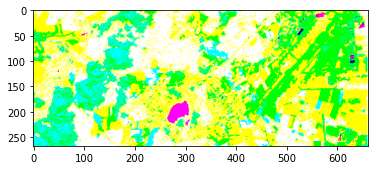
\includegraphics[width=0.65\textwidth]{images/pca_wessling.png}
\end{figure}

We can add an interpretation to the different combination-weights:
\begin{figure}[H]
    \caption{Interpretation of the most important primary components}
    \centering
      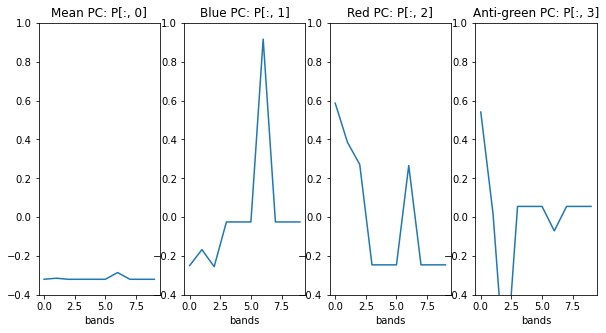
\includegraphics[width=0.65\textwidth]{images/pca_wessling_pcs.png}
\end{figure}




\subsubsection{Maximum-likelihood classifier}
Maximum likelihood is probably the simplest form of supervised learning you can do.
Let's assume that we can group pixels according to their band-values in the groups field, forrest, water, and building.
We want to know the probability of a pixel being in the class 'water', given it's band-values.
\begin{equation}
    P(W|b_1, b_2, b_3, ...) = P(b_1, b_2, b_3 | W) \frac{P(W)}{P(b_1, b_2, b_3)}
\end{equation}
The term $P(b_1, b_2, b_3 | W)$ is our likelihood. When just comparing different probabilities we may ditch the fraction $\frac{P(W)}{P(b_1, b_2, b_3)}$. As such, the simplest classification algorithm could be implemented like this:

\begin{lstlisting}[language=python]
import scipy.stats._multivariate as mult


def getLikelihoodFunction(samples):
    """
        samples: n * b numpy array
            n: nr of samples
            b: nr of bands
    """
    mu = np.mean(samples, axis=0)
    dm = samples - mu
    Cov = dm.transpose() @ dm
    return mult.multivariate_normal(mu, Cov, allow_singular=True)


def maxLikelihoodClassify(labelledData, data):
    """
        labelledData: list of np.arrays
        data: np.array
        All np.arrays of size n * b
            n: nr of samples
            b: nr of bands
    """

    n, b = data.shape
    l = len(labelledData)

    llhs = [
        getLikelihoodFunction(labelSampleData)
        for labelSampleData in labelledData
    ]

    allClassifications = np.zeros((n, l), dtype=np.dtype('float32'))
    for i, llh in enumerate(llhs):
        allClassifications[:, i] = llh.pdf(data)

    maxLlhClasses = np.argmax(allClassifications, axis=1)
    return maxLlhClasses


#%%
waterSamples = allData[190:201, 275:300, :].reshape(11*25, 10)
buildingSamples = allData[170:200, 300:390, :].reshape(30*90, 10)
treesSamples = allData[50:100, 250:300, :].reshape(50*50, 10)
fieldSamples = allData[50:90, 330:360, :].reshape(40*30, 10)
dataLinear = allData.reshape(268*661, 10)


classes = maxLikelihoodClassify([waterSamples, buildingSamples, treesSamples, fieldSamples], dataLinear)
classesImg = classes.reshape(268, 661, 1)
plt.imshow(classesImg, cmap="Set3")
    
\end{lstlisting}


This classifies our Weßling scene quite nicely.
\begin{figure}[H]
    \caption{Supervised classification of Weßling scene using maximum-likelihood}
    \centering
      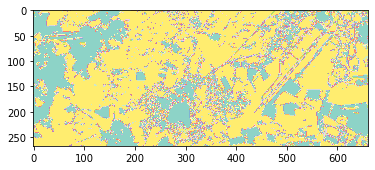
\includegraphics[width=0.65\textwidth]{images/max_likelihood_wessling.png}
\end{figure}





\subsubsection{U-Net}
The U-Net is a popular, convolutional neural net for image segmentation.
\begin{lstlisting}[language=python]
#%%
import os


inputDir = "./data/images"
targetDir = "./data/annotations/trimaps"
imageSize = (160, 160)
numClasses = 3
batchSize = 32

inputImagePaths = sorted([
    os.path.join(inputDir, fName)
    for fName in os.listdir(inputDir)
    if fName.endswith(".jpg")
])

targetImagePaths = sorted([
        os.path.join(targetDir, fName)
    for fName in os.listdir(targetDir)
    if fName.endswith(".png") and not fName.startswith(".")
])

#%% Data-loader

from tensorflow import keras as k
import numpy as np
from tensorflow.keras.preprocessing.image import load_img

class OxfordPets(k.utils.Sequence):
    def __init__(self, batchSize, imgSize, inputImgPaths, targetImgPaths):
        self.batchSize = batchSize
        self.imgSize = imgSize
        self.inputImgPaths = inputImgPaths
        self.targetImgPaths = targetImgPaths

    def __len__(self):
        """ Gives tf the amount of batches available """
        return len(self.targetImgPaths) // self.batchSize

    def __getitem__(self, idx):
        """ Returns tuple (input, target) corresponding to batch #idx """
        i = idx * self.batchSize
        
        batchInputImgPaths = self.inputImgPaths[i : i + self.batchSize]
        batchTargetImgPaths = self.targetImgPaths[i : i + self.batchSize]
        
        x = np.zeros((self.batchSize, self.imgSize[0], self.imgSize[1], 3), dtype='float32')
        for j, path in enumerate(batchInputImgPaths):
            img = load_img(path, target_size=self.imgSize)
            x[j, :, :, :] = img
        
        y = np.zeros((self.batchSize, self.imgSize[0], self.imgSize[1], 1), dtype='uint8')
        for j, path in enumerate(batchTargetImgPaths):
            img = load_img(path, target_size=self.imgSize, color_mode='grayscale')
            y[j] = np.expand_dims(img, 2)
            # Ground truth labels are 1, 2, 3. Subtract one to make them 0, 1, 2:
            y[j] -= 1
        return x, y

    

#%% 
from tensorflow.keras import layers


def makeModel(imgSize, numClasses):
    inputs = k.Input(shape=imgSize + (3,))

    ### First half of model: downsampling inputs

    # Entry block
    x = layers.Conv2D(32, 3, strides=2, padding="same")(inputs)
    x = layers.BatchNormalization()(x)
    x = layers.Activation('relu')(x)
    previousBlockActivation = x

    # Blocks 1, 2, 3 are identical apart from the feature depth
    for filters in [64, 128, 256]:
        x = layers.Activation('relu')(x)
        x = layers.SeparableConv2D(filters, 3, padding='same')(x)
        x = layers.BatchNormalization()(x)
        
        x = layers.Activation('relu')(x)
        x = layers.SeparableConv2D(filters, 3, padding='same')(x)
        x = layers.BatchNormalization()(x)

        x = layers.MaxPooling2D(3, strides=2, padding='same')(x)

        # Project residual
        residual = layers.Conv2D(filters, 1, strides=2, padding='same')(previousBlockActivation)
        x = layers.add([x, residual])
        previousBlockActivation = x  # Setting aside next residual


    ### Second half of network: upsampling inputs

    for filters in [256, 128, 64, 32]:
        x = layers.Activation('relu')(x)
        x = layers.Conv2DTranspose(filters, 3, padding='same')(x)
        x = layers.BatchNormalization()(x)

        x = layers.Activation('relu')(x)
        x = layers.Conv2DTranspose(filters, 3, padding='same')(x)
        x = layers.BatchNormalization()(x)

        x = layers.UpSampling2D(2)(x)

        # Project residual
        residual = layers.UpSampling2D(2)(previousBlockActivation)
        residual = layers.Conv2D(filters, 1, padding='same')(residual)
        x = layers.add([x, residual])
        previousBlockActivation = x

    
    outputs = layers.Conv2D(numClasses, 3, activation='softmax', padding='same')(x)

    model = k.Model(inputs, outputs)
    return model


k.backend.clear_session()

model = makeModel(imageSize, numClasses)
model.summary()


# %%
import random

# Split our img paths into a training and a validation set
val_samples = 1000
random.Random(1337).shuffle(inputImagePaths)
random.Random(1337).shuffle(targetImagePaths)
trainInputImgPaths = inputImagePaths[:-val_samples]
trainTargetImgPaths = targetImagePaths[:-val_samples]
valInputImgPaths = inputImagePaths[-val_samples:]
valTargetImgPaths = targetImagePaths[-val_samples:]

# Instantiate data Sequences for each split
trainGen = OxfordPets(batchSize, imageSize, trainInputImgPaths, trainTargetImgPaths)
validGen = OxfordPets(batchSize, imageSize, valInputImgPaths, valTargetImgPaths)


# %%
# Configure the model for training.
# We use the "sparse" version of categorical_crossentropy
# because our target data is integers.
model.compile(optimizer="rmsprop", loss="sparse_categorical_crossentropy")

callbacks = [
    k.callbacks.ModelCheckpoint("oxford_segmentation.h5", save_best_only=True)
]

# Train the model, doing validation at the end of each epoch.
epochs = 15
model.fit(trainGen, epochs=epochs, validation_data=validGen, callbacks=callbacks)

# %%
valPreds = model.predict(validGen)

\end{lstlisting}